\documentclass[letterpaper,oneside,article,12pt,oldfontcommands]{memoir}

\usepackage{fontspec}
\setmainfont[Ligatures=TeX,Numbers=OldStyle,Numbers=Monospaced]{Alegreya}
\setsansfont[Ligatures=TeX,Numbers=OldStyle,Numbers=Monospaced]{Alegreya Sans}
\setmonofont[Scale=0.8]{Fira Mono}
\setmathtt[Scale=MatchLowercase]{Fira Math}

\usepackage{tikz}[align=flush left]
\usetikzlibrary {arrows,calc,positioning,shapes.misc}
\tikzset{terminal/.style={
    rectangle,minimum size=6mm,rounded corners=2mm,
    very thick,draw=black!50,
    top color=white,bottom color=black!20,
    font=\normalfont}}
\tikzset{every picture/.style={line width=2pt}}

\begin{document}

\noindent{}
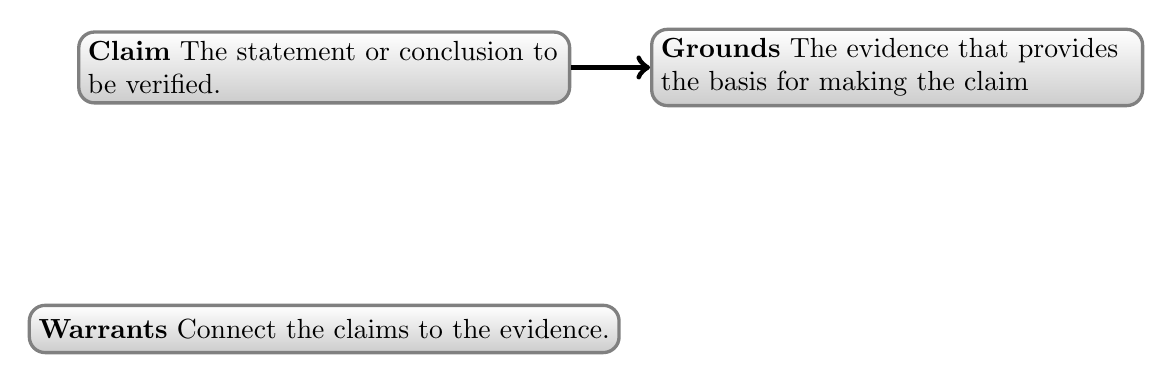
\begin{tikzpicture}[node distance=10mm]
                   
  \node (claim)   [terminal,text width=6cm]                  {\textsc{\textbf{Claim}} The statement or conclusion to be verified.};
  \node (grounds) [terminal,right=of claim,text width=6cm]   {\textsc{\textbf{Grounds}} The evidence that provides the basis for making the claim};
\node (warrant)     [terminal,below=3cm] {\textsc{\textbf{Warrants}} Connect the claims to the evidence.} ;

\draw [->] (claim) -- (grounds);

\end{tikzpicture}

\end{document}

%%% Local Variables:
%%% mode: latex
%%% TeX-master: t
%%% End:
